%%%%%%%%%%%%%%%%%%%%%%%%%%%%%%%%%%%%%%%%%%%%%%%%%%%%%%%%%%%%%%%%%%%%%%%%%%%%%%%
%Tutorial slides on Python.
%
% Author: FOSSEE
% Copyright (c) 2009, FOSSEE, IIT Bombay
%%%%%%%%%%%%%%%%%%%%%%%%%%%%%%%%%%%%%%%%%%%%%%%%%%%%%%%%%%%%%%%%%%%%%%%%%%%%%%%%

\documentclass[14pt,compress]{beamer}
%\documentclass[draft]{beamer}
%\documentclass[compress,handout]{beamer}
%\usepackage{pgfpages}
%\pgfpagesuselayout{2 on 1}[a4paper,border shrink=5mm]

% Modified from: generic-ornate-15min-45min.de.tex
\mode<presentation>
{
  \usetheme{Warsaw}
  \useoutertheme{infolines}
  \setbeamercovered{transparent}
}

\usepackage[english]{babel}
\usepackage[latin1]{inputenc}
%\usepackage{times}
\usepackage[T1]{fontenc}

% Taken from Fernando's slides.
\usepackage{ae,aecompl}
\usepackage{mathpazo,courier,euler}
\usepackage[scaled=.95]{helvet}

\definecolor{darkgreen}{rgb}{0,0.5,0}

\usepackage{listings}
\lstset{language=Python,
    basicstyle=\ttfamily\bfseries,
    commentstyle=\color{red}\itshape,
  stringstyle=\color{darkgreen},
  showstringspaces=false,
  keywordstyle=\color{blue}\bfseries}

%%%%%%%%%%%%%%%%%%%%%%%%%%%%%%%%%%%%%%%%%%%%%%%%%%%%%%%%%%%%%%%%%%%%%%
% Macros
\setbeamercolor{emphbar}{bg=blue!20, fg=black}
\newcommand{\emphbar}[1]
{\begin{beamercolorbox}[rounded=true]{emphbar}
      {#1}
 \end{beamercolorbox}
}
\newcounter{time}
\setcounter{time}{0}
\newcommand{\inctime}[1]{\addtocounter{time}{#1}{\tiny \thetime\ m}}

\newcommand{\typ}[1]{\lstinline{#1}}

\newcommand{\kwrd}[1]{ \texttt{\textbf{\color{blue}{#1}}}  }

\newcommand{\num}{\texttt{numpy}}

%%% This is from Fernando's setup.
% \usepackage{color}
% \definecolor{orange}{cmyk}{0,0.4,0.8,0.2}
% % Use and configure listings package for nicely formatted code
% \usepackage{listings}
% \lstset{
%    language=Python,
%    basicstyle=\small\ttfamily,
%    commentstyle=\ttfamily\color{blue},
%    stringstyle=\ttfamily\color{orange},
%    showstringspaces=false,
%    breaklines=true,
%    postbreak = \space\dots
% }


%%%%%%%%%%%%%%%%%%%%%%%%%%%%%%%%%%%%%%%%%%%%%%%%%%%%%%%%%%%%%%%%%%%%%%
% Title page
\title[NumPy arrays]{Introductory Scientific Computing with
Python}
\subtitle{NumPy arrays}

\author[FOSSEE] {FOSSEE}

\institute[FOSSEE -- IITB] {Department of Aerospace Engineering\\IIT Bombay}
\date[] {Mumbai, India}

%%%%%%%%%%%%%%%%%%%%%%%%%%%%%%%%%%%%%%%%%%%%%%%%%%%%%%%%%%%%%%%%%%%%%%

%\pgfdeclareimage[height=0.75cm]{iitmlogo}{iitmlogo}
%\logo{\pgfuseimage{iitmlogo}}


%% Delete this, if you do not want the table of contents to pop up at
%% the beginning of each subsection:
\AtBeginSubsection[]
{
  \begin{frame}<beamer>
    \frametitle{Outline}
    \tableofcontents[currentsection,currentsubsection]
  \end{frame}
}

\AtBeginSection[]
{
  \begin{frame}<beamer>
    \frametitle{Outline}
    \tableofcontents[currentsection,currentsubsection]
  \end{frame}
}

% If you wish to uncover everything in a step-wise fashion, uncomment
% the following command:
%\beamerdefaultoverlayspecification{<+->}

%\includeonlyframes{current,current1,current2,current3,current4,current5,current6}

%%%%%%%%%%%%%%%%%%%%%%%%%%%%%%%%%%%%%%%%%%%%%%%%%%%%%%%%%%%%%%%%%%%%%%
% DOCUMENT STARTS
\begin{document}

\begin{frame}
  \titlepage
\end{frame}

\begin{frame}
  \frametitle{Outline}
  \tableofcontents
  % You might wish to add the option [pausesections]
\end{frame}


\section{\num\ arrays}

\begin{frame}[fragile]
  \frametitle{The \num\ module}
  \begin{itemize}
  \item Efficient, powerful array type
  \item Abstracts out standard operations on arrays
  \item Convenience functions
  \item \typ{ipython --pylab} imports part of numpy
  \end{itemize}
\end{frame}

\begin{frame}[fragile]
  \frametitle{Without Pylab}
\begin{lstlisting}
In []: from numpy import *
In []: x = linspace(0, 1)
\end{lstlisting}
  Note that we had done this ``import'' earlier!
\begin{lstlisting}
# Can also do this:
In []: import numpy
In []: x = numpy.linspace(0, 1)
# or
In []: import numpy as np
In []: x = np.linspace(0, 1)
\end{lstlisting}
  Note the use of \typ{numpy.linspace}
\end{frame}

\begin{frame}
  \frametitle{\num\ arrays}
  \begin{itemize}
  \item Fixed size (\typ{arr.size})
  \item Same type (\typ{arr.dtype})
  \item Arbitrary dimensionality: \typ{arr.shape}
  \item \typ{shape}: extent (size) along each dimension
  \item \typ{arr.itemsize}: number of bytes per element
  \item \alert{Note:} \typ{shape} can change so long as the \typ{size}
      is constant
  \item Indices start from 0
  \item Negative indices work like lists
  \end{itemize}
\end{frame}

\begin{frame}[fragile]
  \frametitle{\num\ arrays}
\begin{lstlisting}
In []: a = array([1,2,3,4])
In []: b = array([2,3,4,5])

In []: print(a[0], a[-1])
(1, 4)

In []: a[0] = -1
In []: a[0] = 1
\end{lstlisting}
Operations are elementwise
\end{frame}

\begin{frame}[fragile]
  \frametitle{Simple operations}
\begin{lstlisting}
In []: a + b
Out[]: array([3, 5, 7, 9])
In []: a*b
Out[]: array([2, 6, 12, 20])
In []: a/b
Out[]: array([0, 0, 0, 0])
\end{lstlisting}
  \begin{itemize}
  \item Operations are \alert{element-wise}
  \item Types matter
  \end{itemize}
  \inctime{10}
\end{frame}

\begin{frame}[fragile]
  \frametitle{Data type matters}
  Try again with this:
\begin{lstlisting}
In []: a = array([1.,2,3,4])
In []: a/b
\end{lstlisting}
\end{frame}

\begin{frame}[fragile]
  \frametitle{Examples}
\noindent \typ{pi} and \typ{e} are defined.
\begin{lstlisting}
In []: x = linspace(0.0, 10.0, 200)
In []: x *= 2*pi/10
# apply functions to array.
In []: y = sin(x)
In []: y = cos(x)
In []: x[0] = -1
In []: print(x[0], x[-1])
(-1.0, 10.0)
\end{lstlisting}
\end{frame}

\begin{frame}[fragile]
    \frametitle{\typ{size, shape, rank} etc.}
\vspace*{-8pt}
\begin{lstlisting}
In []: x = array([1., 2, 3, 4])
In []: size(x)
Out[]: 4
In []: x.dtype
dtype('float64')
In []: x.shape
Out[] (4,)
In []: rank(x)
Out[]: 1
In []: x.itemsize
Out[]: 8
\end{lstlisting}
\end{frame}


\begin{frame}[fragile]
  \frametitle{Multi-dimensional arrays}
\begin{lstlisting}
In []: a = array([[ 0, 1, 2, 3],
  ...:            [10,11,12,13]])
In []: a.shape # (rows, columns)
Out[]: (2, 4)

In []: a[1,3]
Out[]: 13

In []: a[1,3] = -1
In []: a[1] # The second row
array([10,11,12,-1])
In []: a[1] = 0 # Entire row to zero.
\end{lstlisting}
\inctime{10}
\end{frame}

\subsection{Slicing arrays}

\begin{frame}[plain,fragile]
  \frametitle{Slicing arrays}
  \vspace*{-0.2in}
\begin{lstlisting}
In []: a = array([[1,2,3], [4,5,6],
  ...:            [7,8,9]])
In []: a[0,1:3]
\end{lstlisting}
  \pause
  \vspace*{-0.1in}
\begin{lstlisting}
Out[]: array([2, 3])

In []: a[1:,1:]
\end{lstlisting}
  \pause
  \vspace*{-0.1in}
\begin{lstlisting}
Out[]: array([[5, 6],
                [8, 9]])

In []: a[:,2]
\end{lstlisting}
  \pause
  \vspace*{-0.1in}
\begin{lstlisting}
Out[]: array([3, 6, 9])
\end{lstlisting}
\end{frame}

\begin{frame}[plain,fragile]
  \frametitle{Slicing arrays ...}
  \vspace*{-0.2in}
\begin{lstlisting}
In []: a = array([[1,2,3], [4,5,6],
  ...:            [7,8,9]])

In []: a[0::2,0::2] # Striding...
\end{lstlisting}
  \pause
  \vspace*{-0.1in}
\begin{lstlisting}
Out[]: array([[1, 3],
              [7, 9]])
# Slices refer to the same memory!
\end{lstlisting}
\end{frame}

\subsection{Array creation}

\begin{frame}[fragile]
  \frametitle{Array creation functions}
  \begin{itemize}
  \item \typ{array(object)}
  \item \typ{linspace(start, stop, num=50)}
  \item \typ{ones(shape)}
  \item \typ{zeros((d1,...,dn))}
  \item \typ{empty((d1,...,dn))}
  \item \typ{identity(n)}
  \item \typ{ones\_like(x)}, \typ{zeros\_like(x)}, \typ{empty\_like(x)}
  \end{itemize}
  May pass an optional \typ{dtype=} keyword argument

  For more dtypes see: \typ{numpy.typeDict}

\end{frame}

\begin{frame}[fragile]
  \frametitle{Creation examples}
  \vspace*{-0.25in}
\begin{lstlisting}
In []: a = array([1,2,3], dtype=float)
In []: ones_like(a)
Out[]: array([ 1.,  1.,  1.])

In []: ones( (2, 3) )
Out[]: array([[ 1.,  1.,  1.],
              [ 1.,  1.,  1.]])

In []: identity(3)
Out[]: array([[ 1.,  0.,  0.],
              [ 0.,  1.,  0.],
              [ 0.,  0.,  1.]])
\end{lstlisting}
  \inctime{15}
\end{frame}

\begin{frame}[fragile]
  \frametitle{Array math}
  \begin{itemize}
  \item Basic \alert{elementwise} math (given two arrays \typ{a, b}):
    \begin{itemize}
        \item \typ{a + b} $\rightarrow$ \typ{add(a, b)}
        \item \typ{a - b}, $\rightarrow$ \typ{subtract(a, b)}
        \item \typ{a * b}, $\rightarrow$ \typ{multiply(a, b)}
        \item \typ{a / b}, $\rightarrow$ \typ{divide(a, b)}
        \item \typ{a \% b}, $\rightarrow$ \typ{remainder(a, b)}
        \item \typ{a ** b}, $\rightarrow$ \typ{power(a, b)}
    \end{itemize}
  \item Inplace operators: \typ{a += b}, or \typ{add(a, b,
      a)}
    \alert{What happens if \typ{a} is \typ{int} and \typ{b} is \typ{float?}}
  \end{itemize}
\end{frame}

\begin{frame}[fragile]
  \frametitle{Array math}
  \begin{itemize}
  \item Logical operations: \typ{==, !=, <, >}, etc.
  \item \typ{sin(x), arcsin(x), sinh(x)},
      \typ{exp(x), sqrt(x)} etc.
  \item \typ{sum(x, axis=0), product(x, axis=0)}
  \item \typ{dot(a, b)}
  \end{itemize}
\end{frame}

\begin{frame}[fragile]
    \frametitle{Convenience functions: \typ{loadtxt}}
  \begin{itemize}
      \item \typ{loadtxt(file_name)}: loads a text file
      \item \typ{loadtxt(file_name, unpack=True)}: loads a text file and
          unpacks columns
  \end{itemize}
  \begin{lstlisting}
In []: x = loadtxt('pendulum.txt')
In []: x.shape
Out[]: (90, 2)

In []: x, y = loadtxt('pendulum.txt',
  ...:                 unpack=True)
In []: x.shape
Out[]: (90,)
  \end{lstlisting}

  \inctime{10}
\end{frame}


\begin{frame}[fragile]
  \frametitle{Advanced}
  \begin{itemize}
  \item Only scratched the surface of \num
  \item \typ{reduce, outer}
  \item Typecasting
  \item More functions: \typ{take, choose, where}, \typ{compress,
      concatenate}
  \item Array broadcasting and \typ{None}
  \item Record arrays
  \end{itemize}
\end{frame}

\begin{frame}[fragile]
  \frametitle{Learn more}
  \small
    \begin{itemize}
        \item \url{https://docs.scipy.org/doc/numpy-dev/user/quickstart.html}
        \item \url{http://numpy.org}
    \end{itemize}
\end{frame}

\begin{frame}[fragile]
  \frametitle{Recap}
  \begin{itemize}
      \item Basic concepts: creation, access, operations
      \item 1D, multi-dimensional
      \item Slicing
      \item Array creation, dtypes
      \item Math
      \item \typ{loadtxt}
      \end{itemize}
      \inctime{5}
\end{frame}

\subsection{Example: plotting data from file}

\begin{frame}[fragile]
\frametitle{Example: plotting data from file}
\alert{Data is usually present in a file!} \\
Lets look at the \typ{pendulum.txt} file.
\begin{lstlisting}
In []: cat pendulum.txt
1.0000e-01 6.9004e-01
1.1000e-01 6.9497e-01
1.2000e-01 7.4252e-01
1.3000e-01 7.5360e-01
\end{lstlisting}
\ldots
\end{frame}

\begin{frame}[fragile]
\frametitle{Reading \typ{pendulum.txt}}
\begin{itemize}
  \item File contains L vs.\ T values
  \item First Column - L values
  \item Second Column - T values
  \item Let us generate a plot from the data file
\end{itemize}
\end{frame}

\begin{frame}[fragile]
    \frametitle{Gotcha and an aside}
    Ensure you are in the same directory as \typ{pendulum.txt}\\
    if not, do the following on IPython:
    \begin{lstlisting}
In []: %cd directory_containing_file
# Check if pendulum.txt is there.
In []: ls
# Also try
In []: !ls
    \end{lstlisting}

    \alert{Note:} \typ{\%cd} is an IPython magic command.  For more information
    do:
    \begin{lstlisting}
In []: ?
In []: %cd?
    \end{lstlisting}
\end{frame}


\begin{frame}[fragile]
  \frametitle{Exercise}
  \begin{itemize}
  \item Plot L versus T square with dots
  \item No line connecting points
  \end{itemize}
  \inctime{10}
\end{frame}

\begin{frame}[fragile]
\frametitle{Solution}
\begin{lstlisting}
In []: L, t = loadtxt('pendulum.txt',
 ....:                unpack=True)
In []: plot(L, t*t, '.')
\end{lstlisting}
or
\begin{lstlisting}
In []: x = loadtxt('pendulum.txt')
In []: L, t = x[:,0], x[:,1]
In []: plot(L, t*t, '.')
\end{lstlisting}

\end{frame}


\begin{frame}[fragile]
\begin{figure}
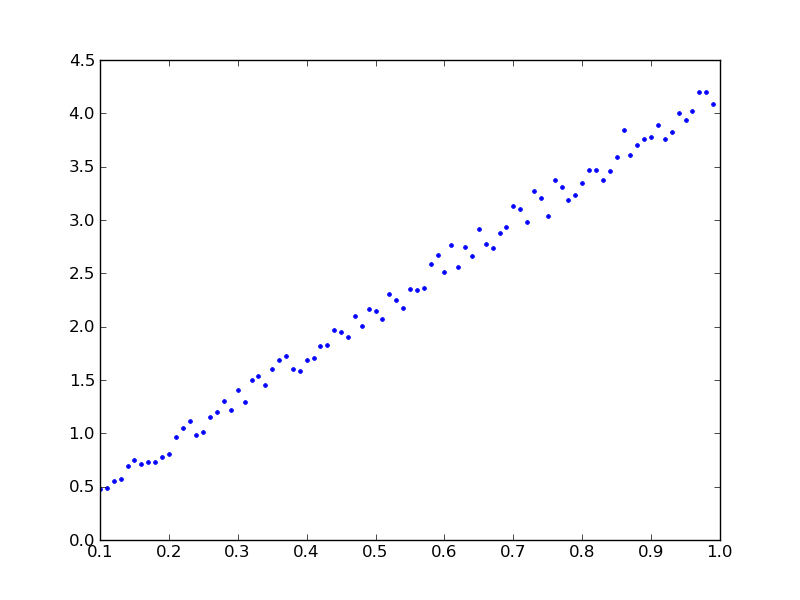
\includegraphics[width=3.5in]{data/L-Tsq.png}
\end{figure}
\end{frame}

\begin{frame}[fragile]
\frametitle{Odds and ends}
\begin{lstlisting}
In []: mean(L)
Out[]: 0.54499999999999993

In []: std(L)
Out[]: 0.25979158313283879
\end{lstlisting}
\end{frame}

\begin{frame}[fragile]
\frametitle{Summary}
\begin{itemize}
\item Introduction to \num\ arrays
\item Slicing arrays
\item Multi-dimensional arrays
\item Array operations
\item Creating arrays
\item Loading data from file
\end{itemize}

\inctime{5}
\end{frame}

\end{document}
